\documentclass[a4paper,11pt]{article}
\usepackage[british]{babel}
\usepackage{fullpage}
\usepackage{amsmath,amssymb}
\usepackage{multirow}
\usepackage{caption}
\usepackage{tikz,pgfplots}
\usepackage{hyperref}
\usepackage{graphicx}
\usepackage{enumitem}
\title{\textbf{Low-level Parallel Programming (course 1DL550) \\
    Uppsala University -- Spring 2015 \\
    Report for Lab 1 by Team 14}}
\author{Fredrik Larsson \and Jimmy Holm \and Per Bergqwist}
\date{\today}
\begin{document}
\maketitle
\section{Plot}
\begin{center}
  \pgfplotsset{grid style={dotted,gray}}
  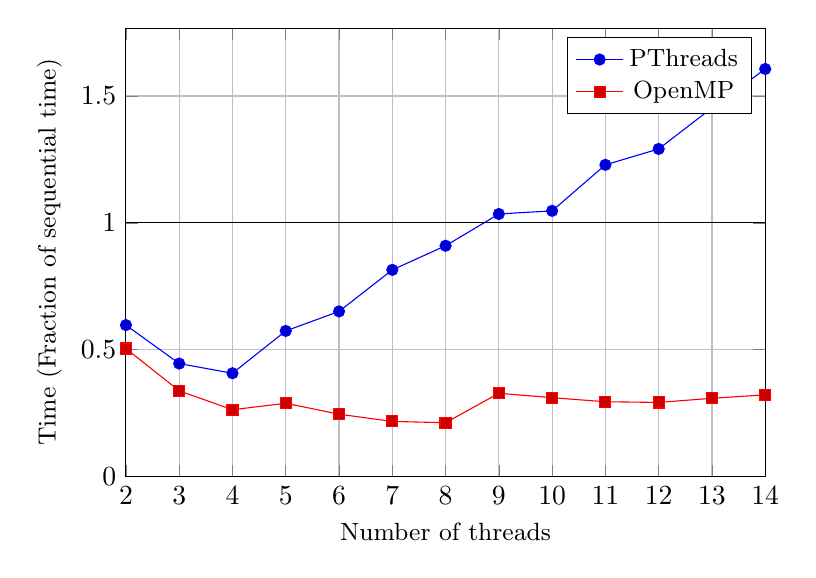
\begin{tikzpicture}
    \begin{axis}[
        width=0.8\textwidth,
        height=0.6\textwidth,
        xtick={2,...,14},
        xmin=2,
        xmax=14,
        ymin=0,
        grid=both,
        legend entries={\small PThreads,\small OpenMP},
        xlabel={\small Number of threads},
        ylabel={\small Time (Fraction of sequential time)}
      ]
      \addplot coordinates{
        (2,0.596941)
        (3,0.445256)
        (4,0.407209)
        (5,0.573977)
        (6,0.650869)
        (7,0.814665)
        (8,0.909659)
        (9,1.0349)
        (10,1.04726)
        (11,1.22862)
        (12,1.29125)
        (13,1.45297)
        (14,1.60644)};
      \addplot coordinates{
        (2,0.504375)
        (3,0.337991)
        (4,0.263352)
        (5,0.288928)
        (6,0.245644)
        (7,0.217354)
        (8,0.21215)
        (9,0.328347)
        (10,0.310834)
        (11,0.294817)
        (12,0.292123)
        (13,0.308487)
        (14,0.322058)};
      \draw (axis cs:2,1) -- (axis cs:14,1);
    \end{axis}
  \end{tikzpicture}
\end{center}
The data used in the plot is the average of 20 runs for each
implementation and is presented as fraction of sequential run-time. A value greater than $1$ indicates
longer run-time than sequential and a value less than $1$ indicates a shorter one.
\section{System specification}
The CPU of the system used for gathering the data presented was an Intel i7 2600k
running at a frequency of 4GHz. The system was able to use four cores
with Hyper-threading enabled, meaning a possibility of using eight logical
cores simultaneously with the drawback that the performance gain from
using more than four cores varies depending on the tasks.
\section{Questions}
\begin{enumerate}[label=\Alph*.]
\item \textbf{What kind of parallelism is exposed in the identified
  method?}\\
  The methods expose data parallelism as it distributes a shared set of data to be processed by the threads.
\item \textbf{How is the workload distributed across the threads?}\\
  For the PThread implementation the workload is distributed uniformly. The agent-vector is divided
  up among the threads in equal parts and each thread work only on their assigned portion of the data.
  The OMP implementation makes use of a threadpool, giving threads which finish their assigned data more data
  to work with until all the data has been processed.
\item \textbf{Which number of thread gives you the best results?
  Why?}\\ 4 or 8 threads gives the best results depending on which
  implementation that was used. OpenMP gives the best performance at eight
  threads while the PThreads implementation at four threads. Our
  conclusion why PThread loses performance with more than four threads is
  because the overhead from our PThreads implementation counter the
  performance gain from the Hyper-threading. OpenMP has the best
  performance at eight threads, however after four threads the gain is
  minimal. When using more than eight threads, which is more than number of
  logical cores available to the CPU, the performance for both OpenMP and PThreads get
  worse and PThread even display worse results than the sequential implementation.
\item \textbf{Which version (OpenMP, Pthreads) gives you better
  results? Why?}\\
  OpenMP produces the best results out of all options, as its use of a thread pool means an
  asymmetric workload does not hinder performance. The PThread solution displays a naive form of sharing as
  it is not certain that each task will finish in an equal amount of time and as such threads that finish their part
  faster, have to wait for the remaining threads to finish up. In OpenMP's implementation, threads that finish can
  take new tasks and as such they are utilized to a greater extent and slower threads do not hold up the larger task.
\end{enumerate}
\section{How to run}
The demo runs with a GUI and using the sequential implementation
if no flag has overwritten the settings. The following flags can be
used to alter the demo and change the implementation for the tick
function.
\begin{itemize}[label=,leftmargin=0pt]
\item \textbf{-\--timing-mode} - Without gui.
\item \textbf{-\--pthread} - Executes the PThread implementation.
\item \textbf{-\--omp} - Executes the OpenMP implementation.
\item \textbf{-\--threads \textit{number}} - Tells the demo to use
  \textit{number} threads when executing.
\item \textbf{-\--silent} - Does not print to standard output.
\item \textbf{-\--plot} - Stores the timing data to the file testdata.txt
\end{itemize}
\section*{Work effort}
All team members put in the same amount of effort on the code and the
report was written by Jimmy and Per with data for the graphs from Per
and Fredrik.
\end{document}
